\begin{exercise}
	Δίνονται τα σημεία $P_1(3, 5), P_2 (9, 18)$ Θεωρώντας ότι το σημείο $P_1$ φωτίζεται στην οθόνη, εφαρμόστε τον αλγόριθμο του Bresenham για τον υπολογισμό των $5$ αμέσως επόμενων pixels που θα φωτισθούν κατα τη σχεδίαση του ευθύγραμμου τμήματος $P_1 P_2$.	
\end{exercise}


\begin{solution}

Όπως έχουμε δει στη θεωρία, προκειμένου να σχεδιάσουμε την ευθεία του Bresenham για σημεία που ανήκουν στο 2ο οκταμόριο, μπορούμε να χρησιμοποιήσουμε τα συμμετρικά των σημείων $P_1, P_2$ ως προς την $1$η διχοτόμο, τα οποία θα ανήκουν στο 1ο οκταμόριο. Άρα θα χρησιμοποιήσουμε τα σημεία $P_1^{'}(5,3)$ και $P_2^{'}(18,9)$ και θα χρησιμοποιήσουμε τον γνωστό αλγόριθμο του Bresenham για σχεδιασμό ευθυγράμμου τμήματος στο 1ο οκταμόριο ως εξής:

\begin{lstlisting}[caption={Αλγόριθμος του Bresenham για 1ο οκταμόριο}]
x1, y1 = get_coordinates("Give the coordinates of P1 e.g. (1,2):")
x2, y2 = get_coordinates("Give the coordinates of P2:")
Dx = x2 - x1
Dy = y2 - y1
x = x1
y = y1
c1 = 2 * Dy
er = c1 - Dx
c2 = er - Dx
while x <= 18
    plot(x, y)
    x = x + 1
    if er < 0
        er = er + c1
    else
        y = y + 1
        er = er + c2
    plot(x, y)
end
\end{lstlisting}


Για τα σημεία \( P_1^{'}(5, 3) \) και \( P_2^{'}(18, 9) \) θα έχουμε:

\begin{itemize}[noitemsep, topsep=0pt] % Reduce vertical spacing
\begin{multicols}{2} % Split into 2 columns
  \item \( x = x_1 = 5 \)
  \item \( y = y_1 = 3 \)
  \item \( \Delta x = x_2 - x_1 = 18 - 5 = 13 \)
  \item \( \Delta y = y_2 - y_1 = 9 - 3 = 6 \)
  \item \( c_1 = 2 \cdot \Delta y = 2 \cdot 6 = 12 \)
  \item \( er = c_1 - \Delta x = 12 - 13 = -1 \)
  \item \( c_2 = er - \Delta x = -1 - 13 = -14 \)
\end{multicols}
\end{itemize}

Ο αλγόριθμος θα τρέξει ως εξής:

\lstset{style=tt} 

\begin{itemize}
  \item \underline{1η επανάληψη}

		\begin{lstlisting}
		x == 5 $<=$ 18 $\Rightarrow$
			plot(5, 3) 
			x = 6 %(x == x + 1) 
			er == -1 $<$ 0 
				er = 11 %(er == er + c1 == -1 + 12 == 11)
		\end{lstlisting}
		
	\item \underline{2η επανάληψη}
		
		\begin{lstlisting}
		x == 6 $\leq$ 18 $\Rightarrow$
			plot(6, 3)
			x = 7 %(x == x + 1 == 7)
			er == 11 $\geq$ 0 
				y = 4 %(y == y + 1 == 4)
				er = -3 %(er == er + c2 == 11 + (-14) == -3)
		\end{lstlisting}		
				
	\item \underline{3η επανάληψη}
		\begin{lstlisting}
		x == 7 $\leq$ 18 $\Rightarrow$
			plot(7, 4)
			x = 8 %(x == x + 1 == 8)
			er == -3 $<$ 0 
				er = 9 %(er == er + c1 == -3 + 12 == 9)
		\end{lstlisting}		
		
	\item \underline{4η επανάληψη}
		\begin{lstlisting}
		x == 8 $\leq$ 18 $\Rightarrow$
			plot(8, 4)
			x = 9 %(x == x + 1 == 9)
			er == 9 $\geq$ 0 
				y = 5 %(y == y + 1 == 5)
				er = -5 %(er == er + c2 == 9 + (-14) == -5)
		\end{lstlisting}
				
	\item \underline{5η επανάληψη}
		\begin{lstlisting}
		x == 9 $\leq$ 18 $\Rightarrow$
			plot(9, 5)
			x = 10 %(x == x + 1 == 10)
			er == -5 $<$ 0 
				er = 7 %(er == er + c1 == -5 + 12 == 7)
		\end{lstlisting}
		
	\item \underline{6η επανάληψη}
		\begin{lstlisting}
		x == 10 $\leq$ 18 $\Rightarrow$
			plot(10, 5)
			x = 11 %(x == x + 1 == 11)
			er == 7 $\geq$ 0 
				y = 6 %(y == y + 1 == 6)
				er = -7 %(er == er + c2 == 7 + (-14) == -7)
		\end{lstlisting}
\end{itemize}

Τα $6$ πρώτα σημεία που θα φωτιστούν δηλαδή από τον αλγόριθμο με είσοδο τις συντεταγμένες $P_1^{'}$ και $P_2^{'}$, είναι: \( (5,3) \to (6, 3) \to (7, 4) \to (8, 4) \to (9, 5) \to (10, 5) \).

Για να βρούμε λοιπόν τα $5$ αμέσως επόμενων pixels που θα φωτισθούν κατα τη σχεδίαση του ευθύγραμμου τμήματος $P_1 P_2$ αρκεί να βρούμε τα συμμετρικά των παραπάνω φωτισμένων pixel ως προς την $1$η διχοτόμο.

Τα ζητούμενα δηλαδή σημεία, δεδομένου ότι θα φωτιστεί το pixel με κέντρο $(3,5)$ θα είναι: \newline 
$(3, 6) \to (4, 7) \to (4, 8) \to (5, 9) \to (5, 10) $

\begin{figure}[hbt]
  \begin{center}
	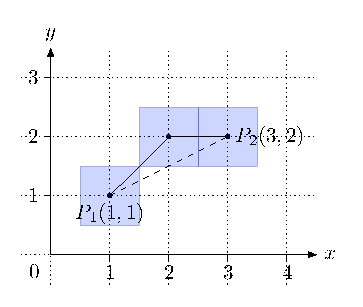
\includegraphics[scale=0.7]{Chapter1/Exercises/ex14/graph1.pdf}
  \end{center}
  \caption{Παράσταση ευθυγράμμων τμημάτων $P_1 P_2$ και $P_1^{'} P_2^{'}$ σύμφωνα με τον αλγόριθμο του Bresenham $P_1(3, 5), P_2 (9, 18)$ για σημεία $P_1^{'}(5, 3), P_2^{'} (18, 9)$}
\end{figure}


\end{solution}